\documentclass[xcolor=svgnames,t]{beamer} 
\usepackage[utf8]{inputenc}
\usepackage{booktabs, comment}
\usepackage{graphicx}  % Add graphicx package
\usepackage[absolute, overlay]{textpos} 
\usepackage{pgfpages}
\usepackage[font=footnotesize]{caption}
\useoutertheme{infolines} 
\usepackage{xcolor}
% \usepackage{cite}  % REMOVE this line because it conflicts with natbib
\usepackage{colortbl}
\definecolor{brownbrown}{RGB}{8, 8, 9}
\usepackage[round, sort, authoryear]{natbib}  % Use only natbib for citation management
\definecolor{brownred}{RGB}{198, 198, 198}

\setbeamercolor{title in head/foot}{bg=brownred, fg=brownbrown}
\setbeamercolor{author in head/foot}{bg=myuniversity}
\setbeamertemplate{page number in head/foot}{}

\usepackage{amsmath}
\usepackage[makeroom]{cancel}

\newtheorem{equi}{} %Creates a grey box when equi is called
\setbeamertemplate{navigation symbols}{} 
\usepackage{textpos}

\usepackage{tikz}

\usetheme{Madrid}
\definecolor{myuniversity}{RGB}{48, 67, 180}
\usecolortheme[named=myuniversity]{structure}
\usepackage{tikz}


\usepackage{colortbl} 
\newcommand{\myitem}{\item[$\circ$]}
\newcommand{\witem}{\item[\textcolor{white}{$\bullet$}]}
\DeclareMathOperator*{\argmax}{arg\,max}
\DeclareMathOperator*{\argmin}{arg\,min}
\AtBeginSection[]{
\begin{frame}
\frametitle{Content}
\tableofcontents[currentsection]
\end{frame}
}

\title[Difference-in-Differences]{Difference-in-Differences}
\subtitle{}
%\titlegraphic{\includegraphics[height=1cm]{brown-logo.png}}  % This line is commented out to remove the logo
\author[CIML ]{Causal Inference using Machine Learning\\ Master in Economics, UNT}
\institute[]{Andres Mena}
\date{Spring 2024}

\addtobeamertemplate{navigation symbols}{}{%
    \usebeamerfont{footline}%
    \usebeamercolor[fg]{footline}%
    \hspace{1em}%
    \insertframenumber/\inserttotalframenumber
}

\begin{document}
\begin{frame}
\maketitle
\end{frame}

\begin{frame}{What is Panel Data?}
    \textbf{Panel Data Definition:}
    \begin{itemize}
        \item Observations for each unit \(i\) (e.g., person, state) across multiple time periods \(t\).
        \item Allows us to account for unobservable characteristics that are constant over time.
        \pause
        \item Example: Gas prices in neighborhoods with and without Thrifty stations, observed before and after a merger.
    \end{itemize}
    \centering
    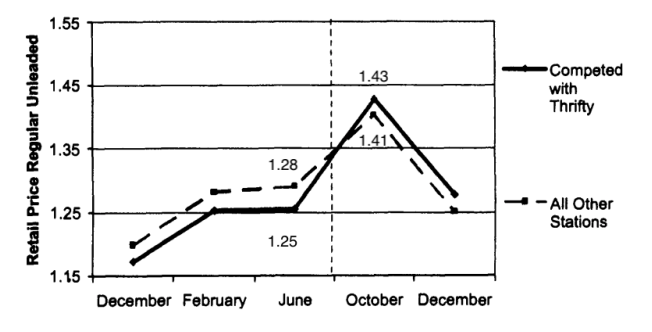
\includegraphics[width=0.6\textwidth]{Figures/hastings_example.png}
    \end{frame}
    
    \begin{frame}{Defining Treatment in Panel Data}
    \begin{itemize}
        \item \textbf{Treatment Definition:}
        \begin{itemize}
            \item Let \(Y_{it}\) be the outcome for unit \(i\) at time \(t\).
            \item \(D_i = 1\): Treated units.
            \item \(D_i = 0\): Control units.
        \end{itemize}
        \pause
        \item \textbf{Key Assumptions:}
        \begin{itemize}
            \item No anticipation: Treatment in \(t\) does not affect outcomes in earlier periods.
            \item Parallel trends: Control and treatment groups would have followed the same trend in the absence of treatment.
        \end{itemize}
    \end{itemize}
    \end{frame}
    
    \begin{frame}{Conditional Expectations Before and After Treatment}
    \begin{itemize}
        \item \textbf{Observed Outcomes:}
        \begin{equation*}
        Y_{it} = G_{it} Y_{it}(1) + (1 - G_{it}) Y_{it}(0)
        \end{equation*}
        
        \item \textbf{Parallel Trends Assumption}
        \begin{equation*}
            E[Y_{it}(0) - Y_{it-j}(0) | D_i = 1] = E[Y_{it}(0) - Y_{it-j}(0) | D_i = 0]
        \end{equation*}
        \pause
        \item \textbf{No anticpation}\\
         \[
        E(Y_{it}|D_i=1)=E(Y_{it}(0)|D_i=1) \quad \text{for all } t<T
        \] \pause
        \item \textbf{Average Treatment on The treated}
        \begin{equation*}
        E[Y_{it}(1) - Y_{it}(0) | D_i = 1]
        \end{equation*}
    \end{itemize}
    \end{frame}
    
    \begin{frame}{Identification in Differences-in-Differences (DiD) - Part 1}
        \textbf{Step-by-Step Setup}
        \begin{itemize}
            \item \textbf{Notation:} 
            \begin{itemize}
                \item $Y_{it}$: Observed outcome for unit $i$ at time $t$.
                \item $D_i$: Treatment indicator ($D_i=1$ if treated, $D_i=0$ if control).
            \end{itemize}
    
            \item \textbf{Simple Difference (Within-Group Change):}
            \[
            \Delta Y_i = Y_{i2} - Y_{i1}.
            \]
            \[
            E[\Delta Y_i | D_i=1] = E[Y_{i2}-Y_{i1} | D_i=1],
            \quad
            E[\Delta Y_i | D_i=0] = E[Y_{i2}-Y_{i1} | D_i=0].
            \]
    
            \item \textbf{Double Difference (Between-Group Change):}
            \[
            \text{DiD} = \big(E[Y_{i2} | D_i=1]-E[Y_{i1} | D_i=1]\big) - \big(E[Y_{i2} | D_i=0]-E[Y_{i1} | D_i=0]\big).
            \]
        \end{itemize}
    \end{frame}
    
    \begin{frame}{Identification in DiD - Part 1}
        \small
        
        \[
        \text{DiD} = \bigl[ E(Y_{2}|D=1) - E(Y_{1}|D=1) \bigr] - \bigl[ E(Y_{2}|D=0) - E(Y_{1}|D=0) \bigr].
        \]
        
        \textbf{Potential Outcomes:}
        \begin{equation*}
            Y_{it} = G_{it} Y_{it}(1) + (1 - G_{it}) Y_{it}(0)
        \end{equation*}
        
        \textbf{Replacing Observed with Potential Outcomes:}\\
        - For $D_i=1$ and $t=2$: $E(Y_{i2}|D_i=1)=E(Y_{i2}(1)|D_i=1)$. \\
        - For $D_i=1$ and $t=1$: $E(Y_{i1}|D_i=1)=E(Y_{i1}(0)|D_i=1)$. (No Anticipation) \\
        - For $D_i=0$: $E(Y_{it}|D_i=0)=E(Y_{it}(0)|D_i=0)$ for all $t$
        
        Thus:
        \[
        \text{DiD} = \bigl[E(Y_{2}(1)|D=1)-E(Y_{1}(0)|D=1)\bigr] - \bigl[E(Y_{2}(0)|D=0)-E(Y_{1}(0)|D=0)\bigr].
        \]
        \end{frame}
        
        \begin{frame}{Identification in DiD - Part 2}
        \small
        \textbf{Substrac and Add $E(Y_{2}(0)|D=1)-E(Y_{1}(0)|D=1)$:}
        \[
        \text{DiD} = \underbrace{\bigl[E(Y_{2}(1)-Y_{2}(0)|D=1)\bigr]}_{\text{ATT}}
        \]
        \[
            + \underbrace{\bigl[E(Y_{1}(0)-Y_{1}(0)|D=1)\bigr]}_{\text{=0}}
            \]
        \[
        + \underbrace{\bigl[E(Y_{2}(0)-Y_{1}(0)|D=1)-E(Y_{2}(0)-Y_{1}(0)|D=0)\bigr]}_{\text{Selection Bias}}.
        \]
        
        \pause
        \textbf{Parallel Trends Assumption:}
        \[
        E(Y_{2}(0)-Y_{1}(0)|D=1)=E(Y_{2}(0)-Y_{1}(0)|D=0) \implies \text{Selection Bias}=0.
        \]
        \pause
        \textbf{Conclusion:}
        \[
        \text{DiD}=E(Y_{2}(1)-Y_{2}(0)|D=1)=\text{ATT}.
        \]
        \end{frame}
        
        
    
    
    
    \begin{frame}{Two-Way Fixed Effects Model}
    \textbf{Regression Specification:}
    \begin{equation*}
    Y_{it} = \beta_0 + \beta_1 \text{Post}_t + \beta_2 D_i + \beta_3 (D_i \times \text{Post}_t) + \epsilon_{it}
    \end{equation*}
    \pause
    \textbf{Coefficients:}
    \begin{itemize}
        \item \(\beta_0\): Baseline outcome for control group in pre-treatment period.
        \item \(\beta_1\): Time trend for control group.
        \item \(\beta_2\): Baseline difference between treated and control groups.
        \item \(\beta_3\): Treatment effect (DiD estimate).
    \end{itemize}
    \pause
    \textbf{Extensions:}
    \begin{itemize}
        \item Add unit and time fixed effects to control for unobserved heterogeneity.
    \end{itemize}
    \end{frame}
    
    \begin{frame}{Example: Hastings (2004)}
    \begin{itemize}
        \item Studied gas price changes after ARCO's merger with Thrifty.
        \item Pre-treatment: Gas stations in areas competing with Thrifty had prices 3 cents lower.
        \item Post-treatment: Prices in treated areas increased by 2 cents.
    \end{itemize}
    \centering
    \pause
    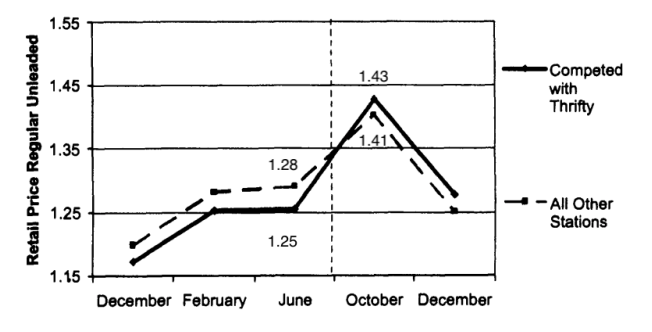
\includegraphics[width=0.6\textwidth]{Figures/hastings_example.png}
    \pause
    
    \begin{align*}
    \text{Effect} &= \text{Post-treatment difference} - \text{Pre-treatment difference} \\
        &= 2 - (-3) = 5 \text{ cents}
    \end{align*}
    
    
    \end{frame}
    \begin{frame}{Inference in DiD: Clustered Standard Errors}
        \small
        \[
        \widehat{V}_{\text{cluster}}(\hat{\beta}) 
        = (X^{\top}X)^{-1}\left(\sum_{g=1}^{G}X_{g}^{\top}\widehat{\epsilon}_{g}\widehat{\epsilon}_{g}^{\top}X_{g}\right)(X^{\top}X)^{-1},
        \]
        where $g$ indexes clusters, $\widehat{\epsilon}_{g}$ are residuals within cluster $g$, and $X_{g}$ is the design matrix for cluster $g$.
        \end{frame}
        
    \begin{frame}{Conclusion}
    \begin{itemize}
        \item DiD is a powerful tool for causal inference in panel data.
        \pause
        \item Assumptions: Parallel trends and no anticipation.
        \pause
        \item Two-way fixed effects extend DiD to handle more complex settings.
        \pause
        \item Inferences should use standard errors that account for clustering.
    \end{itemize}
    \end{frame}
\end{document}


































 


